\section{Experiments}
[Dataset and annotation, evaluation and numerical results]

{\bf Dataset and Annotation:} We have experimented with multiple edge detectors including Canny~\cite{canny}, Pb~\cite{martin2004} 
and Crisp boundary~\cite{isola14crisp} edge detectors, and finally settled down on the Pb edge detector for our purposes. As noted 
before, the choice of edge detector does not significantly affect the computation of unary potentials and the label assignment. 
However, the connected contour nature of Pb edges makes it easier to define the graph connectivity for MRF formulation. Edge 
detection is followed by edge linking to obtain a set of possible edge contour segments in the image. While this approach provides 
good results, it can be readily replaced by any edge detection algorithm that performs well for the given class of 
images~\cite{edgeDetectSurvey-Koschan}.

\begin{figure}[ht]
   \centering
   \subfigure[RGB]{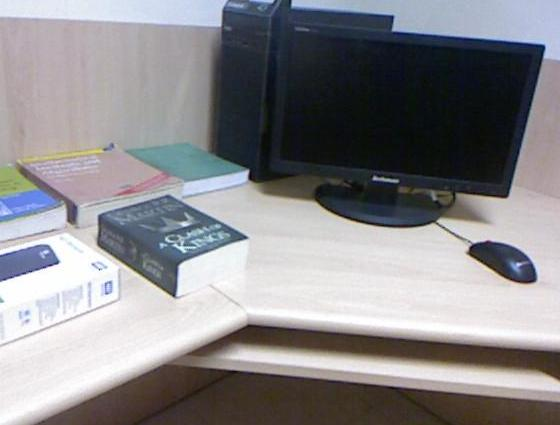
\includegraphics[width=0.25\columnwidth]{results/274.jpg}} \hfill
   \subfigure[Depth Map]{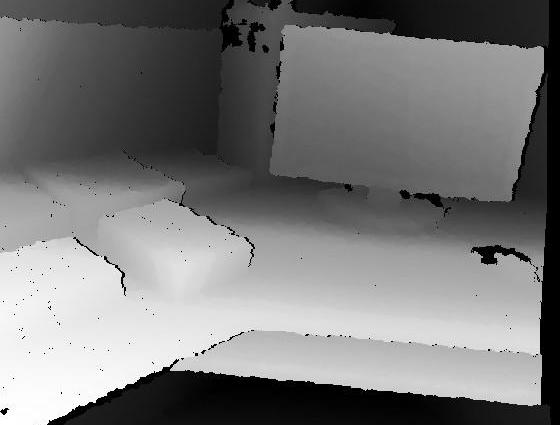
\includegraphics[width=0.25\columnwidth]{results/274_depth.jpg}} \hfill
   \subfigure[Ground truth]{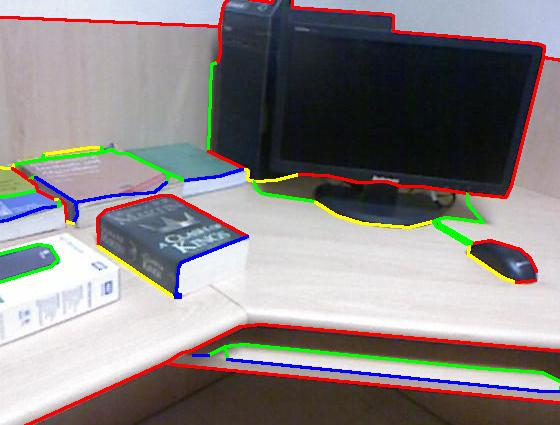
\includegraphics[width=0.25\columnwidth]{results/274_gt.jpg}} \hfill
   \caption{\it Sample image from our dataset showing the RGB image, depth map
   and edge groundtruth. Colors: red (occ), green (pln), blue (cvx), yellow (ccv).}
\label{fig:dataset_depth_GT}
\end{figure}

For quantitative evaluation of the method, we have created an annotated dataset of $500$ RGBD images
of varying complexity. Train to test ratio is 3:2. Though in principle we could use a variety of methods 
to create 3D cues, we use Kinect based images and depth maps in this work. Kinect does not work beyond a 
distance of around four meters. Therefore, our dataset consists of indoor scenes where the objects lie within 
this distance. Our dataset consists of objects such as tables, chairs, cupboard shelves, boxes and household 
objects in addition to walls and floors. We also annotate 100 images from NYU~\cite{Silberman:ECCV12} dataset, 
which include varying scenes from bed-room, living-room, kitchen, bathroom and so on with different complexities. 

For each edge contour, we annotate each of its contour segments with one of the four labels: occlusion, 
convex, concave and planar. The average number of occlusion, planar, convex and concave edges pixels in 
an image in the annotated dataset are $953, 1324, 304$ and $468$ respectively. The corresponding numbers 
for NYU dataset are $1645, 445, 325$ and $399$ respectively. Figure~\ref{fig:dataset_depth_GT} shows an 
annotated example from our dataset. 

\subsection{Evaluation and Numerical Results}

We use recall, precision and F-measure in order to evaluate the performance of the labeling algorithms. 
The average precision, recall and F-measure for each of the edge labels over all the images in the dataset 
is given in Table~\ref{table:evaluation} in addition to results on the NYU dataset. Results for different 
images using the algorithm are given in Figure~\ref{fig:comp2} and Figure~\ref{fig:comp}.

\begin{table}[h]
\begin{center}
\caption{\it Precision, Recall and F-measure for each edge type on our and NYU datasets. $1^{st}$ and $2^{nd}$ 
rows of each set gives the results of our approach and comparison with ~\cite{gupta13Perceptual}. The $3^{rd}$ 
row in each set shows the results of our approach on NYU dataset.}
\label{table:evaluation}
       \begin{tabular}{|c||c|c|c|c|}
       \hline
        & Occluding & Planar & Convex & Concave \\ 
        \hline 
        \hline
	Recall & {\bf 0.85} & {\bf 0.92} & {\bf 0.70} & {\bf 0.78} \\ \hline 
	Gupta {\em et al.}~\cite{gupta13Perceptual} Recall & 0.70 & 0.84 & 0.52 & 0.67 \\ \hline 
	Our Recall on NYU & $0.76$ & $0.85$ & $0.56$ & $0.69$ \\ \hline  \hline
	Precision &  {\bf 0.86 } & {\bf 0.81} & {\bf 0.93} &{\bf 0.89} \\ \hline 
	Gupta {\em et al.}~\cite{gupta13Perceptual} Precision & 0.71 & 0.75 & 0.72 & 0.71 \\ \hline
	Our Precision on NYU & $0.79$ & $0.80$ & $0.77$ & $0.71$ \\ \hline   \hline
	F-measure & {\bf 0.86 } &  {\bf 0.86 } &  {\bf 0.80 } &  {\bf 0.83 } \\ \hline 
	Gupta {\em et al.}~\cite{gupta13Perceptual} F-measure & 0.71 & 0.79 & 0.61 & 0.69 \\ \hline 
	Our F-measure on NYU & $0.77$ & $0.83$ & $0.65$ & $0.70$ \\ \hline 
\end{tabular}
\end{center}
\end{table}
\vspace{-5mm}

\begin{table}[h]
\parbox{.4\linewidth}{
\centering
\caption{\it Confusion matrix across the four classes.  The numbers given
are the average number of edge pixels per image.}
\label{table:confusion}
       \begin{tabular}{|c||c|c|c|c|}
       \hline
        & Occ & Pln & Cvx & Ccv \\ 
        \hline 
        \hline
	Occ & 677 & 100 & 5 & 11 \\ \hline 
	Pln & 53 & 993 & 10 & 27 \\ \hline 
	Cvx & 27 & 58 & 201 & 2 \\ \hline 
	Ccv & 28 & 70 & 1 & 344 \\ \hline 
\end{tabular}
}
\hfill
\parbox{.55\linewidth}{
\centering
\caption{\it Precision, recall and F-measure for each edge type without and with
pairwise potentials.}
\label{table:compare}
       \begin{tabular}{|c||c|c|c|c|}
       \hline
        & Occ & Pln & Cvx & Ccv \\ 
        \hline 
        \hline
	Pixel Recall & 0.82 & 0.87 & 0.69 & 0.75 \\ \hline 
%	Contour Recall & -.-- & -.-- & -.-- & -.-- \\ \hline 
	Final Recall & {\bf 0.85} & {\bf 0.92} & {\bf 0.70} & {\bf 0.78} \\ \hline \hline
	Pixel Precision & 0.84 & {\bf 0.85} & 0.90 &  0.86 \\ \hline 
%	Contour Precision & -.-- & -.-- & -.-- & -.-- \\ \hline 
	Final Precision & {\bf 0.86} &  0.81 & {\bf 0.93} & {\bf 0.89} \\ \hline \hline
	Pixel F-measure & 0.83 & 0.86 & 0.78 & 0.80 \\ \hline 
%	Contour F-measure & -.-- & -.-- & -.-- & -.-- \\ \hline 
	Final F-measure & {\bf 0.86} & {\bf 0.86} & {\bf 0.80} & {\bf 0.83} \\ \hline 
\end{tabular}
}
\end{table}

To understand the effect of unary versus pairwise potentials on the precision and recall measures, we
look at the effect of classification of edge pixels and edge contour segments using only the unary potentials,
without the pairwise terms. Table~\ref{table:compare} shows the resulting precision, recall and F-score
values over the whole database. For convenience of comparison, we have also included the results using
the pairwise terms. We get an average F-score of 0.82 on the classification results for our 
data set. The use of smoothness constraints in the MRF achieves an F-score of 0.84.

We compare the proposed approach with the semantic labeling of edges obtained by 
Gupta {\em et al.}~\cite{gupta13Perceptual}, by computing their results on our dataset of annotated 
edges. Note that their work provides three labels (occluding, convex and concave). Since our dataset 
contains planar edges also, we perform a straight-forward extension of their approach to $4$ labels 
for a fair comparison.

For evaluation purposes, we consider only those pixels in the cropped range $41-600\times46-470$ to 
remove the area where depth information is mostly missing in the Kinect depth map. This was done to 
be consistent with \cite{gupta13Perceptual} in the data used for comparison. Figure~\ref{fig:comp2}, 
Figure~\ref{fig:comp} and table~\ref{table:evaluation} provide qualitative and quantitative comparisons 
of the outputs of the two approaches. It can be seen that our approach produces superior results. 
We see that our approach labels the edges correctly even when they occur extremely close to another type of edge. For \textit{e.g.}, in result (d) of figure~\ref{fig:comp}, the rightmost convex edge got correctly 
classified while the approach by Gupta {\em et al.}~\cite{gupta13Perceptual} fails to do so. Similar results 
can be seen in much of the complex images in the NYU dataset (see figure~\ref{fig:nyuResults}). 

We see that the algorithm achieves high precision for each of the edge types. The recalls are also 
high except for convex and concave edges. This is primarily due to the fact that we have several complex 
scenes in our dataset where a convex/concave edge does not have good depth quantization or do not have 
enough depth values registered around it. We are able to correctly classify complex convex/concave edges 
even with narrow regions having steep slope on either sides of the edge, provided the depth map is good. 
The NYU dataset contains complex scenes with glass windows and table heads for which Kinect fails to 
register the depth accurately. While this results in lower recall for convex and concave edges, we 
achieve an average F-score of $0.74$ for the NYU dataset.

On detailed analysis, the primary causes of errors in our approach were found to be: i) missing depth 
values from Kinect and ii) very small depth differences for occluding edges. While the first problem may 
be solved using better sensors and using image based potentials, the second would require a higher level 
understanding of the scene and objects. The proposed algorithm can be extended to work with SFM point 
clouds as well. The depth map in SFM can be easily created using the camera matrices of images and the 
point cloud. The main challenge here is that SFM point cloud is sparser than Kinect. Therefore, the depth 
and normal information may not be as reliable as that of Kinect.

\begin{figure*}[ht]
   \centering

   \subfigure{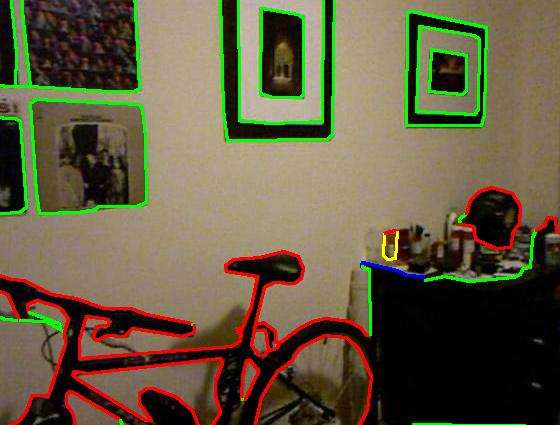
\includegraphics[width=0.19\columnwidth]{results/557_GT.jpg}} \hfill
   \subfigure{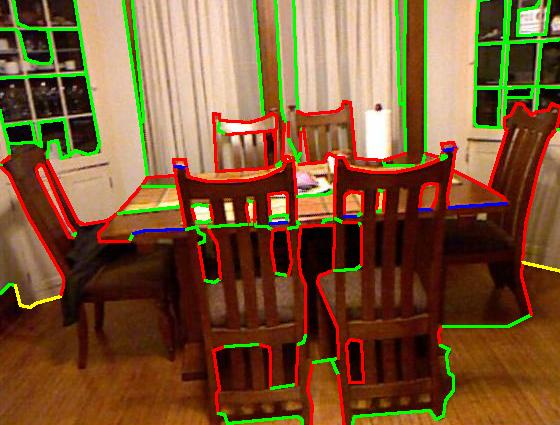
\includegraphics[width=0.19\columnwidth]{results/637_GT.jpg}} \hfill
   \subfigure{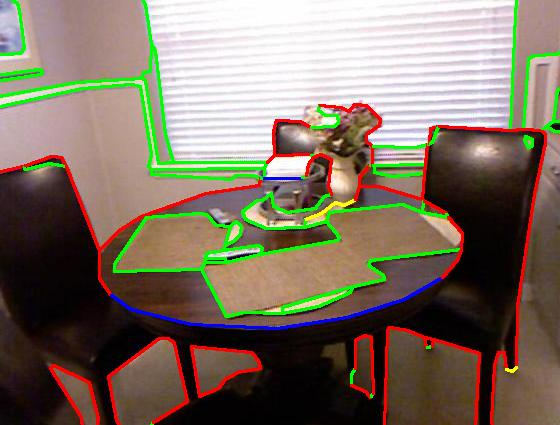
\includegraphics[width=0.19\columnwidth]{results/734_GT.jpg}} \hfill
   \subfigure{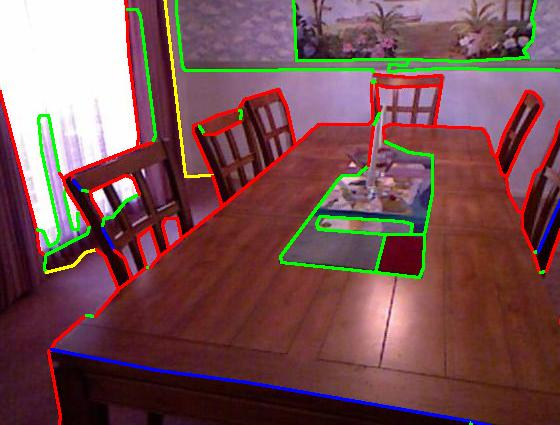
\includegraphics[width=0.19\columnwidth]{results/941_GT.jpg}} \hfill
   \subfigure{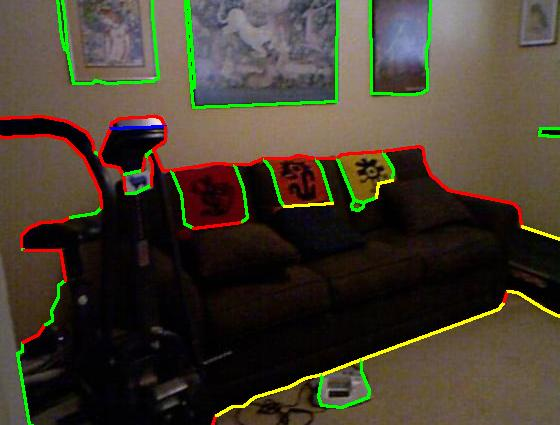
\includegraphics[width=0.19\columnwidth]{results/934_GT.jpg}} \\
   \addtocounter{subfigure}{-5}
   \subfigure{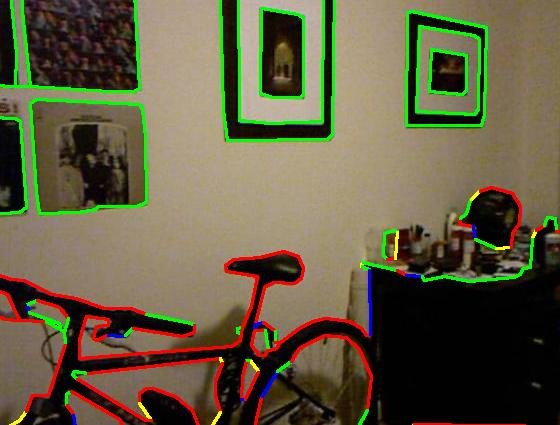
\includegraphics[width=0.19\columnwidth]{results/557_MRF.jpg}} \hfill
   \subfigure{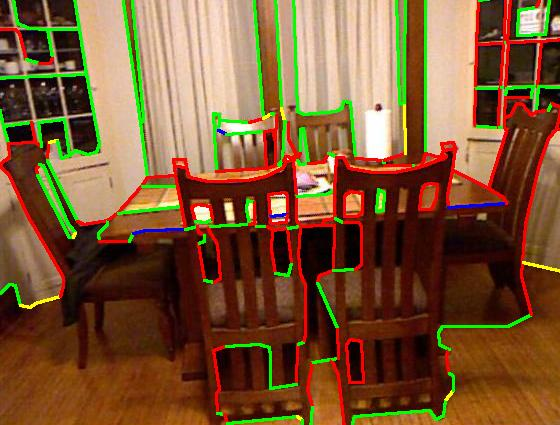
\includegraphics[width=0.19\columnwidth]{results/637_MRF.jpg}} \hfill
   \subfigure{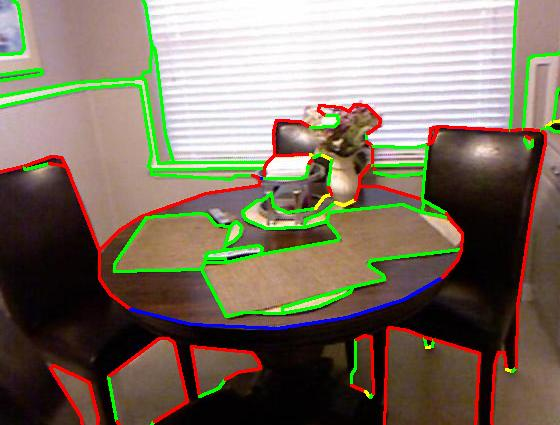
\includegraphics[width=0.19\columnwidth]{results/734_MRF.jpg}} \hfill
   \subfigure{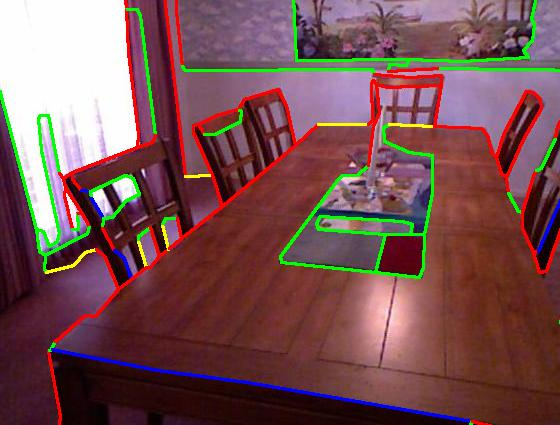
\includegraphics[width=0.19\columnwidth]{results/941_MRF.jpg}} \hfill
   \subfigure{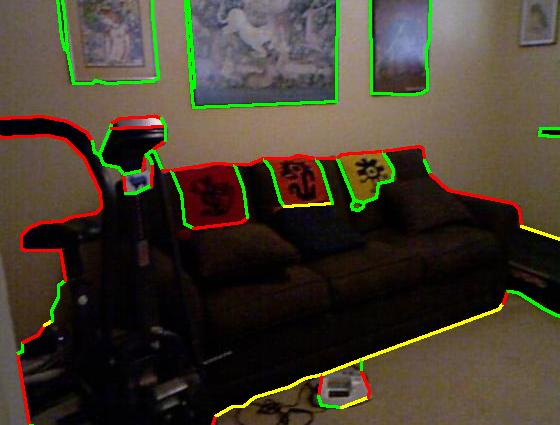
\includegraphics[width=0.19\columnwidth]{results/934_MRF.jpg}} \\
   \addtocounter{subfigure}{-5}

   \caption{\it NYU dataset results : Ground truths (above) and the corresponding results from our approach (below).
   Color code: red (occ), green (pln), blue (cvx), yellow (ccv).}
\label{fig:nyuResults}
\end{figure*}

   \begin{figure*}[ht]
   \centering


   \subfigure{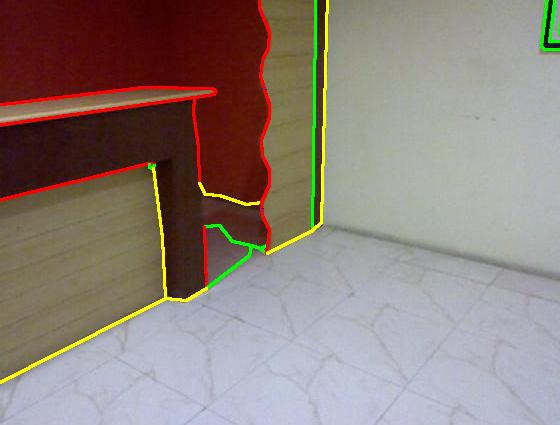
\includegraphics[width=0.16\columnwidth]{results/143_gt.jpg}} \hfill
    \subfigure{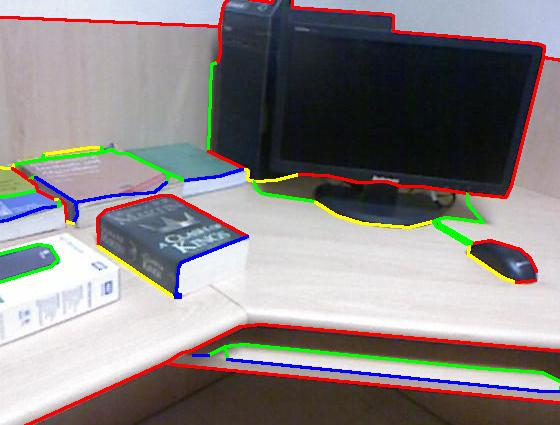
\includegraphics[width=0.16\columnwidth]{results/274_gt.jpg}}  \hfill
   \subfigure{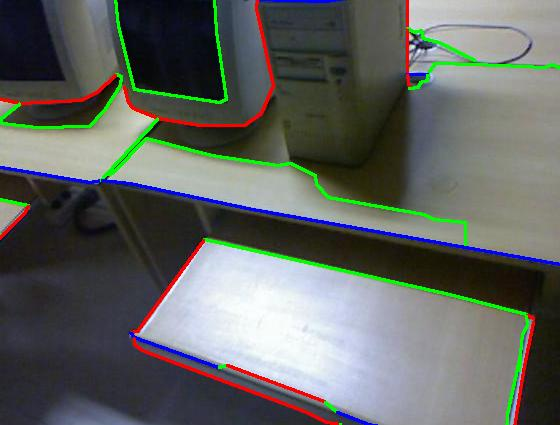
\includegraphics[width=0.16\columnwidth]{supplementary/364_gt.jpg}} \hfill
  \subfigure{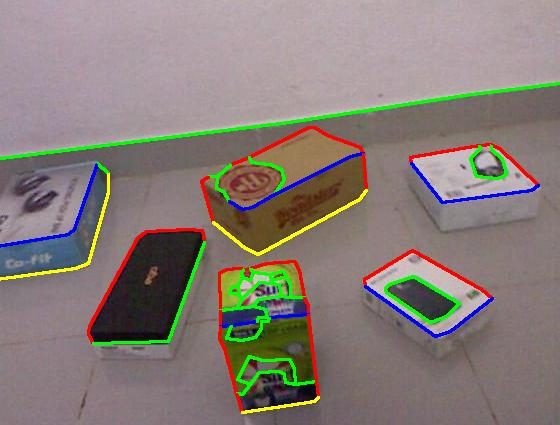
\includegraphics[width=0.17\columnwidth]{results/214_gt.jpg}} \hfill
   \subfigure{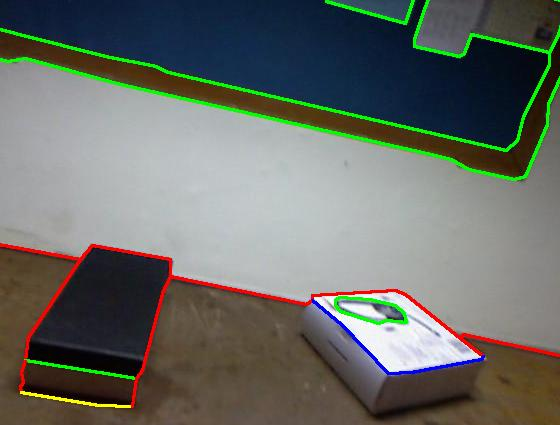
\includegraphics[width=0.17\columnwidth]{supplementary/90_gt.jpg}} \\   
  \subfigure{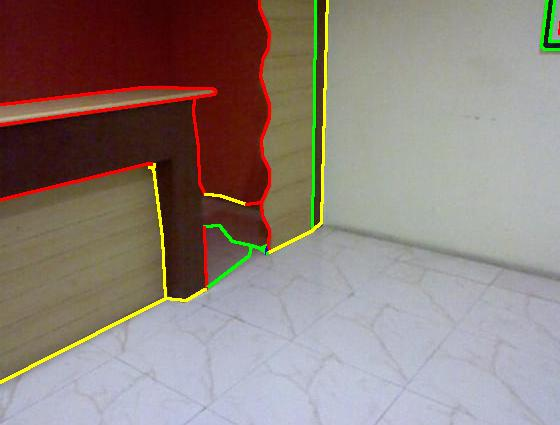
\includegraphics[width=0.16\columnwidth]{results/143_graphcut.jpg}} \hfill
   \subfigure{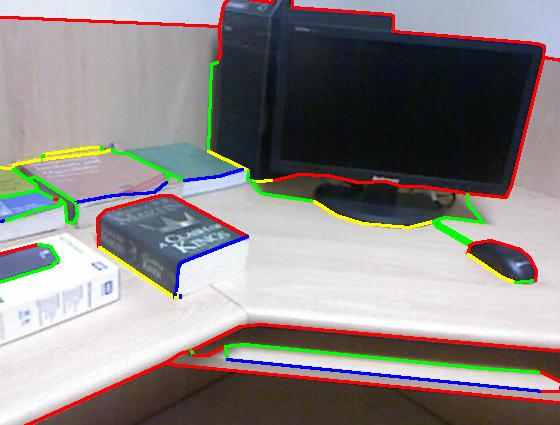
\includegraphics[width=0.16\columnwidth]{results/274_graphcut.jpg}} \hfill
   \subfigure{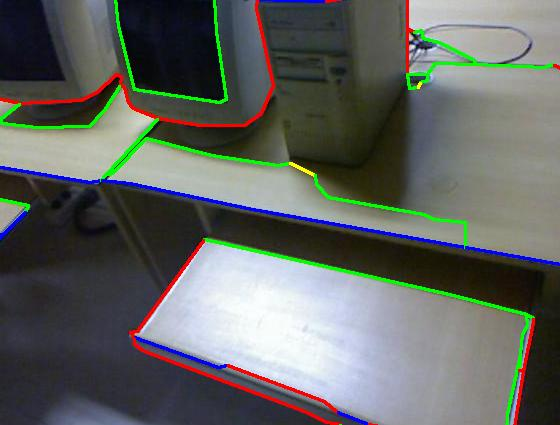
\includegraphics[width=0.16\columnwidth]{supplementary/364_graphcut.jpg}} \hfill
   \subfigure{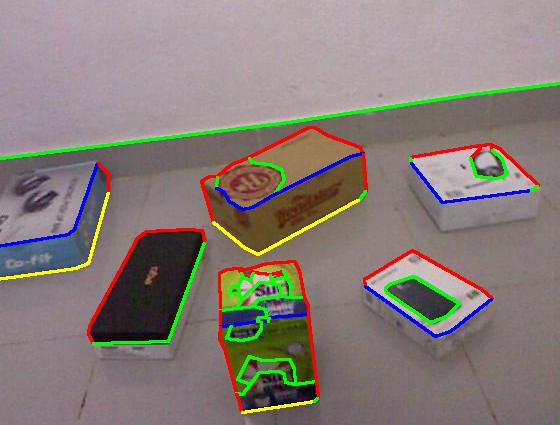
\includegraphics[width=0.17\columnwidth]{results/214_graphcut.jpg}} \hfill
   \subfigure{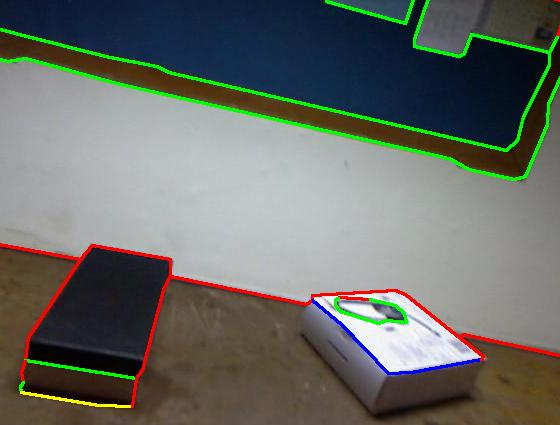
\includegraphics[width=0.17\columnwidth]{supplementary/90_graphcut.jpg}} \\ 
   \addtocounter{subfigure}{-5}
   \subfigure[]{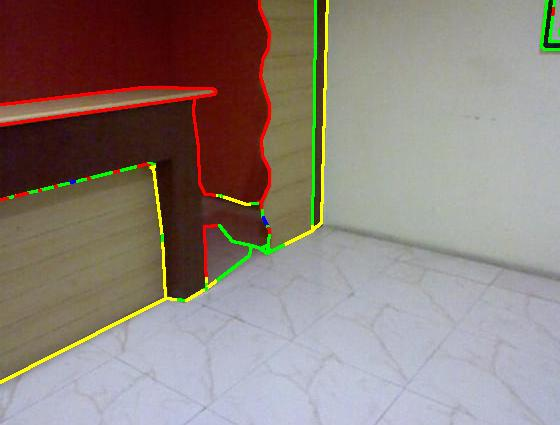
\includegraphics[width=0.16\columnwidth]{results/Gupta/143.jpg}} \hfill
  \subfigure[]{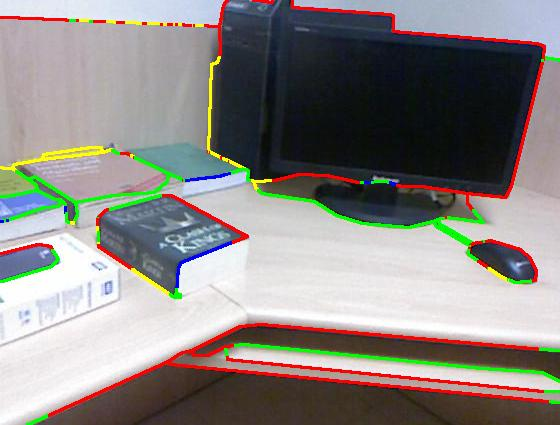
\includegraphics[width=0.16\columnwidth]{results/Gupta/274.jpg}} \hfill
  \subfigure[]{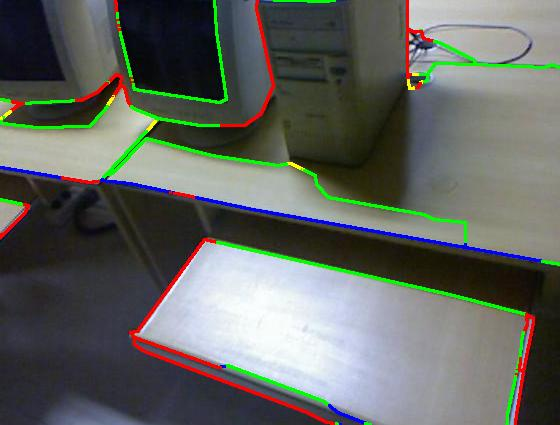
\includegraphics[width=0.16\columnwidth]{results/Gupta/364.jpg}} \hfill
    \subfigure[]{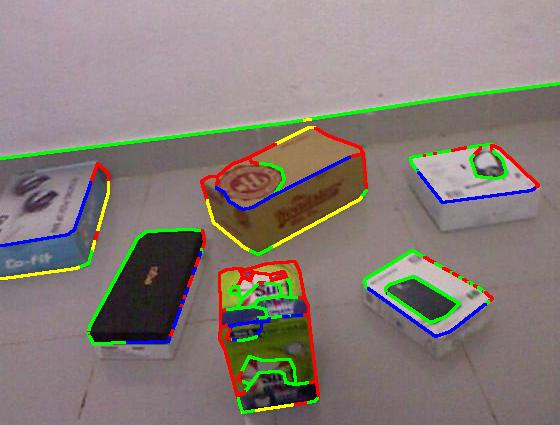
\includegraphics[width=0.17\columnwidth]{results/Gupta/214.jpg}}  \hfill
   \subfigure[]{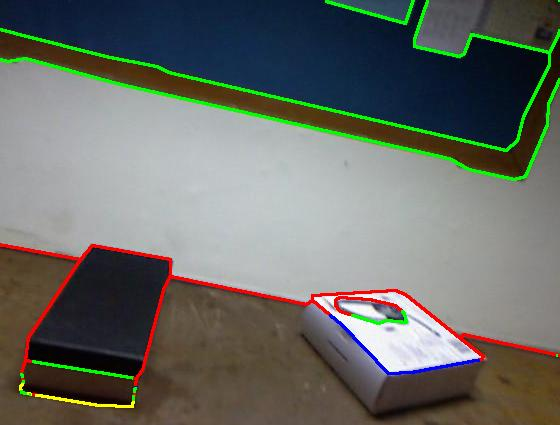
\includegraphics[width=0.17\columnwidth]{results/Gupta/90.jpg}} \\
  \caption{\it Ground truths (above) and the corresponding results from our approach ($2^{nd}$ row)
   and Gupta {\em et al.}~\cite{gupta13Perceptual} ($3^{rd}$ row). Color code: red (occ), green (pln), 
   blue (cvx), yellow (ccv).}
\label{fig:comp2}
\end{figure*}

\begin{figure*}[ht]
   \centering

   \subfigure{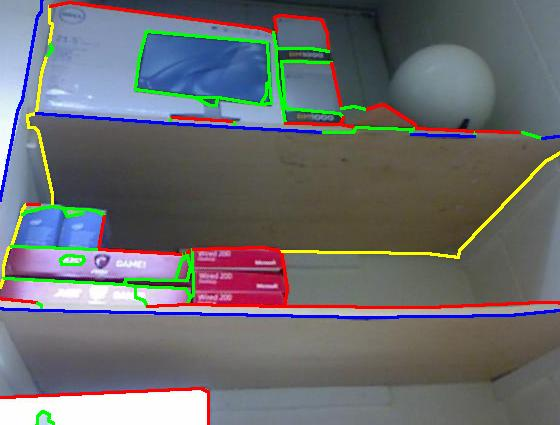
\includegraphics[width=0.19\columnwidth]{results/387_GT.jpg}} \hfill
   \subfigure{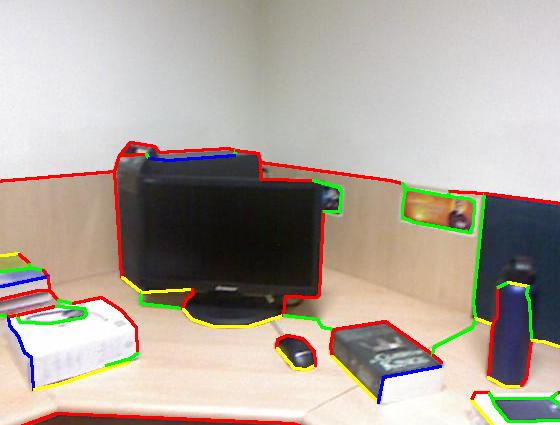
\includegraphics[width=0.19\columnwidth]{results/248_GT.jpg}} \hfill
   %\subfigure{\includegraphics[width=0.19\columnwidth]{results/332_GT.jpg}} \hfill
   \subfigure{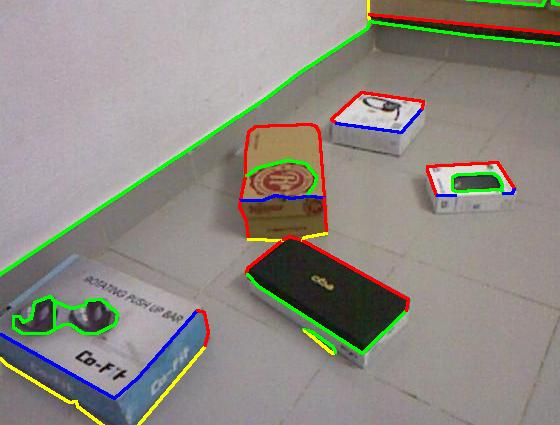
\includegraphics[width=0.19\columnwidth]{results/228_GT.jpg}} \hfill
   \subfigure{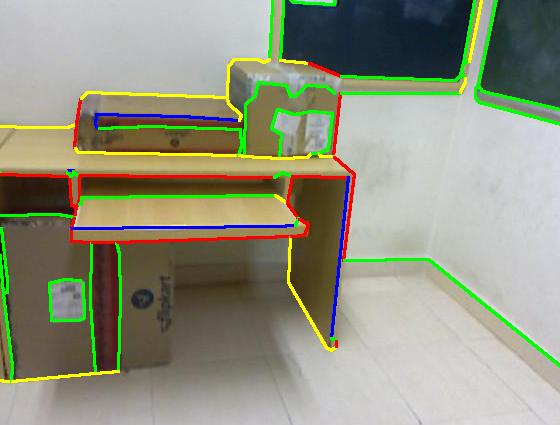
\includegraphics[width=0.19\columnwidth]{results/410_GT.jpg}} \hfill
   %\subfigure{\includegraphics[width=0.19\columnwidth]{results/432_GT.jpg}} \hfill
   \subfigure{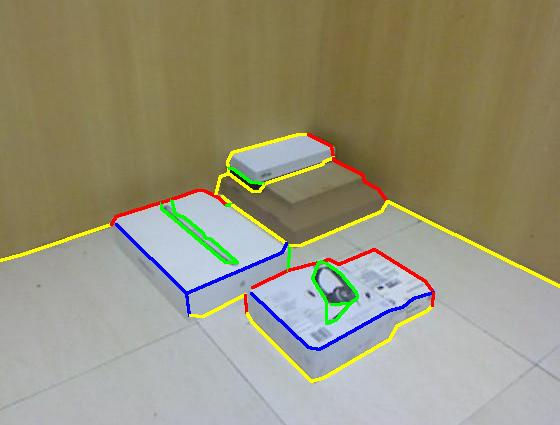
\includegraphics[width=0.19\columnwidth]{results/464_GT.jpg}} \\

   \subfigure{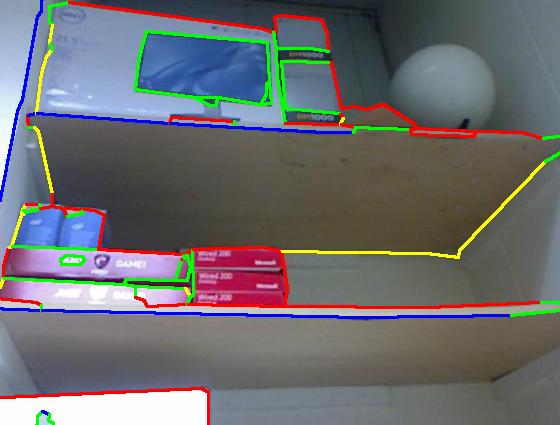
\includegraphics[width=0.19\columnwidth]{results/387_MRF.jpg}} \hfill
   \subfigure{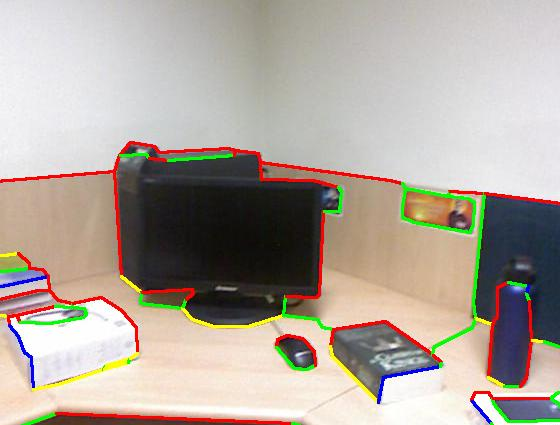
\includegraphics[width=0.19\columnwidth]{results/248_MRF.jpg}} \hfill
   %\subfigure{\includegraphics[width=0.19\columnwidth]{results/332_MRF.jpg}} \hfill
   \subfigure{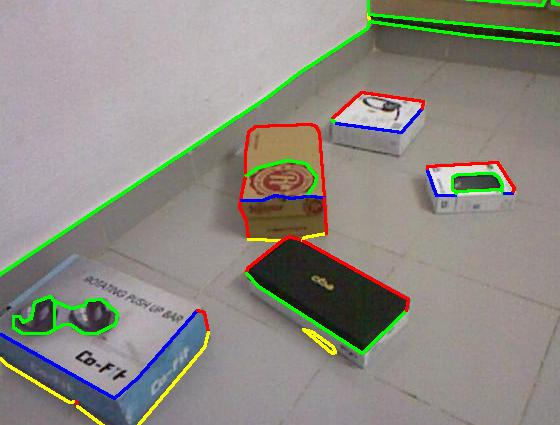
\includegraphics[width=0.19\columnwidth]{results/228_MRF.jpg}} \hfill
   \subfigure{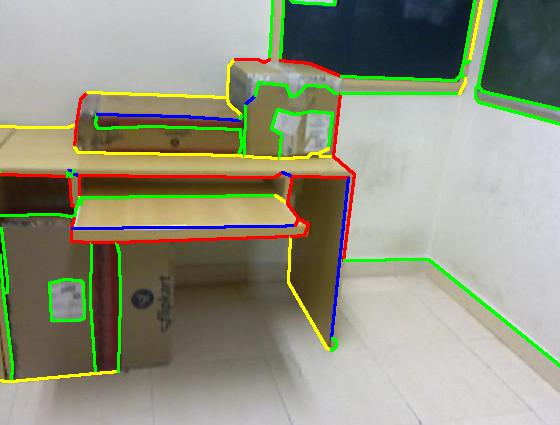
\includegraphics[width=0.19\columnwidth]{results/410_MRF.jpg}} \hfill
   %\subfigure{\includegraphics[width=0.19\columnwidth]{results/432_MRF.jpg}} \hfill
   \subfigure{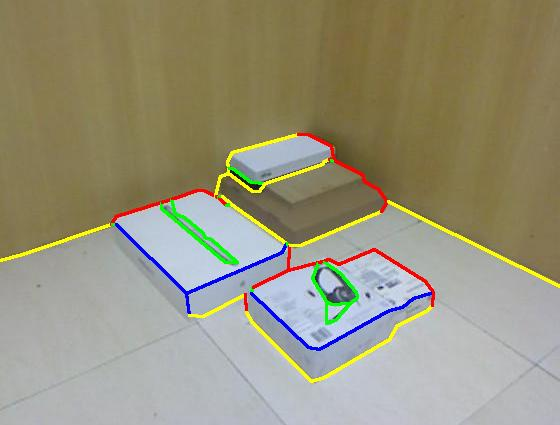
\includegraphics[width=0.19\columnwidth]{results/464_MRF.jpg}} \\ 
   \addtocounter{subfigure}{-10}
   \subfigure[]{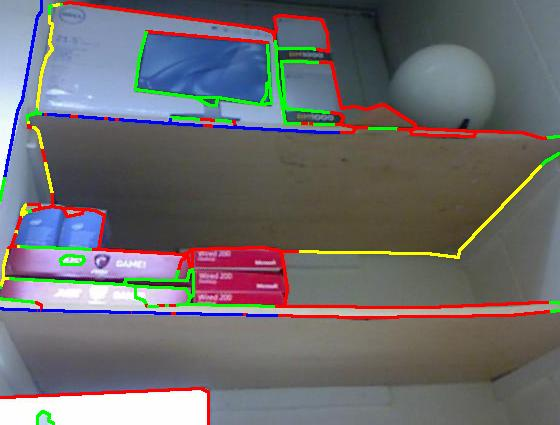
\includegraphics[width=0.19\columnwidth]{results/Gupta/387.jpg}} \hfill
   \subfigure[]{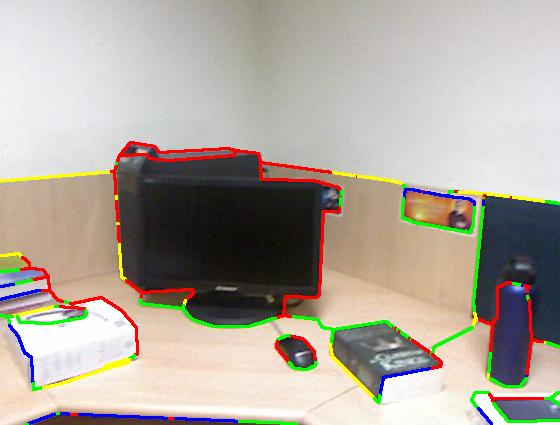
\includegraphics[width=0.19\columnwidth]{results/Gupta/248.jpg}} \hfill
   %\subfigure[]{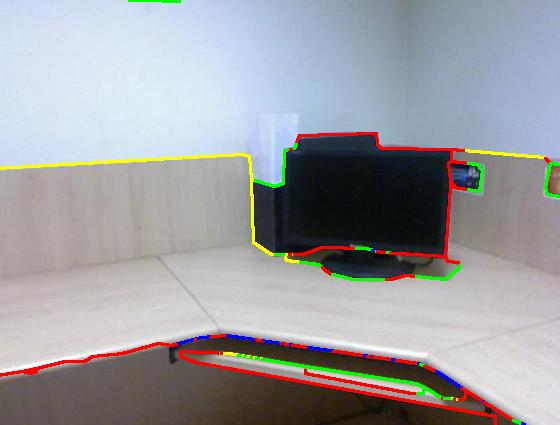
\includegraphics[width=0.19\columnwidth]{results/Gupta/332.jpg}} \hfill
   \subfigure[]{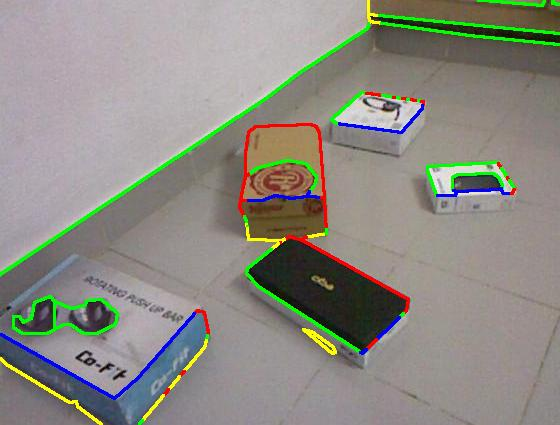
\includegraphics[width=0.19\columnwidth]{results/Gupta/228.jpg}} \hfill
   \subfigure[]{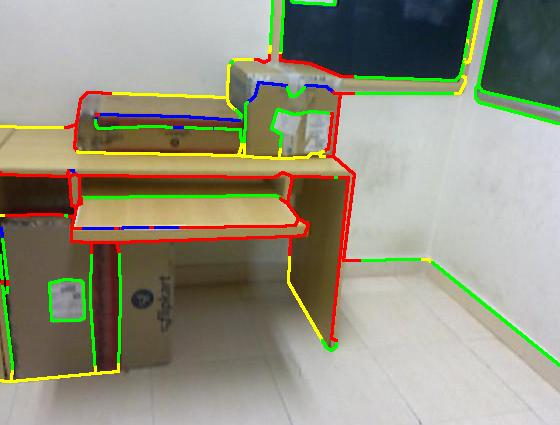
\includegraphics[width=0.19\columnwidth]{results/Gupta/410.jpg}} \hfill
   %\subfigure[]{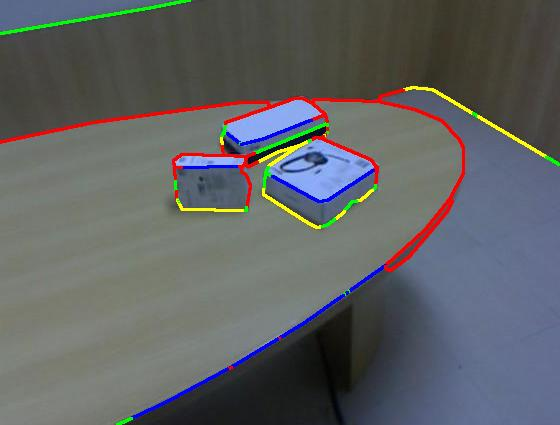
\includegraphics[width=0.19\columnwidth]{results/Gupta/432.jpg}} \hfill
   \subfigure[]{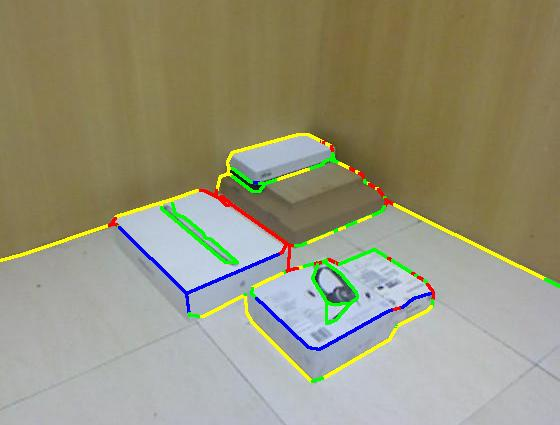
\includegraphics[width=0.19\columnwidth]{results/Gupta/464.jpg}} \\ 

   \subfigure{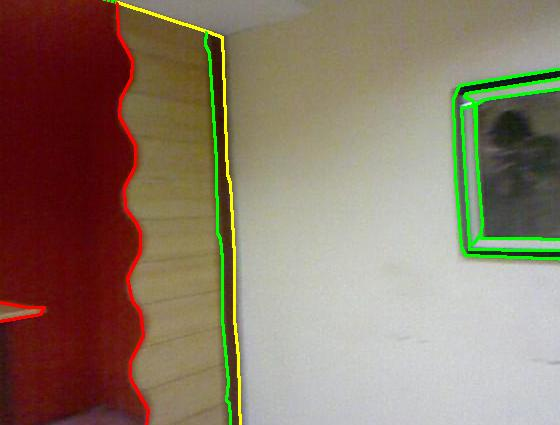
\includegraphics[width=0.17\columnwidth]{supplementary/131_gt.jpg}} \hfill
   \subfigure{\includegraphics[width=0.17\columnwidth]{supplementary/394_gt.jpg}} \hfill
   \subfigure{\includegraphics[width=0.17\columnwidth]{supplementary/407_gt.jpg}} \hfill
  \subfigure{\includegraphics[width=0.17\columnwidth]{supplementary/56_gt.jpg}} \hfill
   \subfigure{\includegraphics[width=0.17\columnwidth]{supplementary/432_gt.jpg}} \\   
   \subfigure{\includegraphics[width=0.17\columnwidth]{supplementary/131_graphcut.jpg}} \hfill
   \subfigure{\includegraphics[width=0.17\columnwidth]{supplementary/394_graphcut.jpg}} \hfill
   \subfigure{\includegraphics[width=0.17\columnwidth]{supplementary/407_graphcut.jpg}} \hfill
   \subfigure{\includegraphics[width=0.17\columnwidth]{supplementary/56_graphcut.jpg}} \hfill
   \subfigure{\includegraphics[width=0.17\columnwidth]{supplementary/432_graphcut.jpg}} \\ 
   \addtocounter{subfigure}{-10}
   \subfigure[]{\includegraphics[width=0.17\columnwidth]{results/Gupta/131.jpg}} \hfill
   \subfigure[]{\includegraphics[width=0.17\columnwidth]{results/Gupta/394.jpg}} \hfill
   \subfigure[]{\includegraphics[width=0.17\columnwidth]{results/Gupta/407.jpg}} \hfill
    \subfigure[]{\includegraphics[width=0.17\columnwidth]{results/Gupta/56.jpg}}  \hfill
   \subfigure[]{\includegraphics[width=0.17\columnwidth]{results/Gupta/432.jpg}} \\
  \caption{\it Ground truths (above) and the corresponding results from our approach ($2^{nd}$ row)
   and Gupta {\em et al.}~\cite{gupta13Perceptual} ($3^{rd}$ row). Color code: red (occ), green (pln), 
   blue (cvx), yellow (ccv).}
\label{fig:comp}
\end{figure*}
